\documentclass[a4paper,12pt]{report}
\usepackage[pdftex]{graphicx}
\graphicspath{{picaa/}}
\usepackage{listings}
\usepackage{amsmath}
\usepackage[T2A]{fontenc}
\usepackage[utf8]{inputenc}
\usepackage[english,russian]{babel}
\usepackage{pgfplots} 

\usepackage{geometry}
\geometry{left=2cm}
\geometry{right=1.5cm}
\geometry{top=1cm}
\geometry{bottom=2cm}
\lstset{language = Python,
	keywordstyle = \color{orange},
	stringstyle = \color{green},
	commentstyle = \color{red},
	columns = fullflexible,
	captionpos = t
}
\begin{document}

    \begin{titlepage}

        \begin{center}
            \large
            \textbf{Государственное образовательное учреждение высшего профессионального образования\\
            “Московский государственный технический университет имени Н.Э.Баумана”\\}
            
\includegraphics{bmstu-logo.png}
			\vspace{1cm}
            
            \textsc{Дисциплина: Анализ алгоритмов}
            \vspace{0.5cm}
                
            \textsc{Лабораторная работа №2}
            \vspace{1cm}
            
            {\LARGE \textbf{Исследование сложности алгоритмов умножения матриц}}
            \vspace{3cm}
                    
            \begin{flushright}
            	Студент группы ИУ7-55Б,\\   
            	Руднев К. К.,\\
            	\vspace{0.5cm}
            	Преподаватель,\\
            	Волкова Л. Л.,\\
            	Строганов Ю. В.
            	
            \end{flushright}
            \vfill
            
            2019 г.
            
            \end{center}

    \end{titlepage}

	\setcounter{page}{2}
	\tableofcontents
    \chapter*{Введение}

		Цель работы: изучение алгоритмов умножения матриц. 
		В данной лабораторной работе рассматривается стандартный алгоритм умножения матриц, алгоритм Винограда и оптимизированный алгоритм Винограда. 
		Также требуется изучить расчет сложности алгоритмов, получить навыки в улучшении алгоритмов.
		
		Задачи:
		\begin{itemize}
			\item изучить алгоритмы умножения матриц: стандартный и алгоритм Винограда;
			\item оптимизировать алгоритм Винограда;
			\item дать теоритическую оценку базового алгоритма матриц, алгоритма Винограда и оптимизированного алгоритма Винограда;
			\item реализовать алгоритмы умножения матриц на одном из языков программирования;
			\item сравнить время работы алгоритмов.
		\end{itemize}
	\label{sec:intro}

    \newpage

    \chapter{Аналитическая часть}
        \label{sec:analitic_part}

			В рамках раздела будет дано аналитическое описание алгоритма для умножения матриц стандартным методом и по Винограду.

	\section{Описание алгоритмов}
        
			Пусть даны две прямоугольные матрицы A[MxQ] и B[QxN]:\\
			A = $\begin{bmatrix}
				a_{11}& a_{12}& ...& a_{1Q}\\
				a_{21}& a_{22}& ...& a_{1Q}\\
				.& .& .& .\\
				.& .& .& .\\
				.& .& .& .\\
				a_{M1}& a_{M2}& ...& a_{MQ}\\
			\end{bmatrix}$, B = $\begin{bmatrix}
				b_{11}& b_{12}& ...& b_{1N}\\
				b_{21}& b_{22}& ...& b_{1N}\\
				.& .& .& .\\
				.& .& .& .\\
				.& .& .& .\\
				b_{Q1}& b_{Q2}& ...& b_{QN}\\
			\end{bmatrix}$ .
			
			\vspace{0.3cm}
			Тогда матрица C[MxN]:\\
			C = $\begin{bmatrix}
				c_{11}& c_{12}& ...& c_{1N}\\
				c_{21}& c_{22}& ...& c_{1N}\\
				.& .& .& .\\
				.& .& .& .\\
				.& .& .& .\\
				c_{M1}& c_{M2}& ...& c_{MN}\\
			\end{bmatrix}$, в которой:\\
			
			\vspace{0.3cm}
			\begin{multline}
				\label{func:std}
				c_{ij} = \sum\limits_{r=1}^m a_{ir}*b_{rj} \ (i=1,2,...M; j=1,2,...N).
			\end{multline} называется их произведением \cite{Beloysov}.\\
			
			\vspace{0.6cm}
			
			\begin{center}
				Алгоритм Винограда
			\end{center}
		
			Пусть даны две прямоугольные матрицы A[1xQ] и B[Qx1]:\\
			U = $\begin{bmatrix}
			u_{1}& u_{2}& ...& u_{Q}\\
			\end{bmatrix}$, V = $\begin{bmatrix}
			v_{1}\\
			v_{2}\\
			.&\\
			.&\\
			.&\\
			v_{Q}\\
			\end{bmatrix}$ .
			
			\vspace{0.3cm}
			Тогда матрица C[1x1] = A*B по формуле \ref{func:vinograd} \cite{Gall2012}:\\
			\begin{multline}
				\label{func:vinograd}
				C_{ij} = u_{1}*v_{1}+u_{1}*v_{1}+...+u_{Q}*v_{Q} =\\ (u_{1}+v_{2})\cdot(u_{2}+v_{1})+...+(u_{Q-2}+v_{Q-2})*(u_{Q}+v_{Q})-\\
				u_{1}*u_{2}-u_{Q-3}*u_{Q-2}-u_{Q-1}*u_{Q}-v_{1}*v_{2}-\\
				v_{Q-3}*v_{Q-2}-v_{Q-1}*v_{Q}
			\end{multline}
			
			В случае, если матрица имеет нечетную размерность, необходимо отдельно обработать последний вектор (формула \ref{func:vinograd_end}):
			\begin{multline}
			\label{func:vinograd_end}
			C_{ij} = u_{in-1}*v_{n-1j}
			\end{multline}
    
    \section{Вывод}

    		Были рассмотрены алгоритмы классического умножения матриц и алгоритм Винограда, основное отличие которых - наличие предварительной обработки, что позволяет снизить количество операций умножения.

    \newpage

   \chapter{Конструкторская часть}
        \label{sec:construct_part}

			В рамках раздела на рисунках \ref{ris:std1}-\ref{ris:wino5} будут представлены схемы алгоритмов стандартного умножения и алгоритма умножения матриц по Винограду.

	\section{Разработка алгоритмов}

		Схема стандартного алгоритма умножения матриц представлена на рисунках \ref{ris:std1}-\ref{ris:std2}.\\
		Схема алгоритма умножения матриц по Винограду представлена на рисунках \ref{ris:wino1}-\ref{ris:wino5}.

	\begin{figure}[h!]
		\centering
		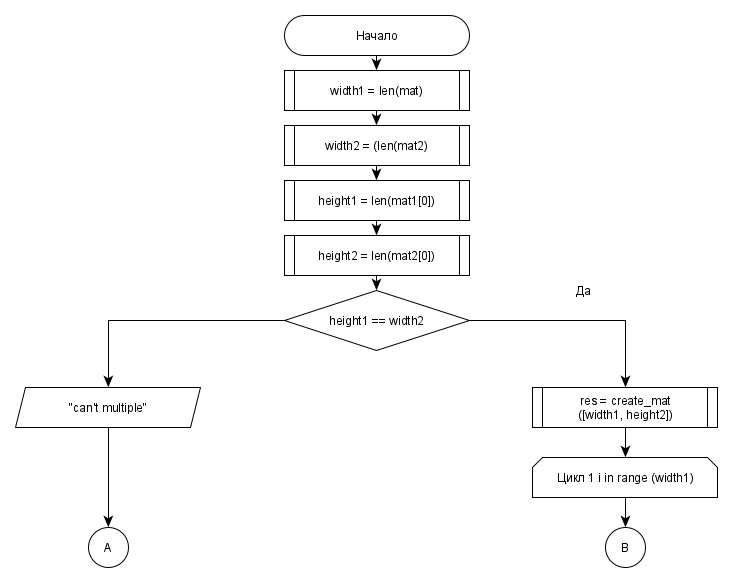
\includegraphics[width=0.8\linewidth]{basedab111.png}
		\caption{Стандартный алгоритм умножения матриц. Часть 1}
		\label{ris:std1}
	\end{figure}

	\newpage

	\begin{figure}[h!]
		\centering
		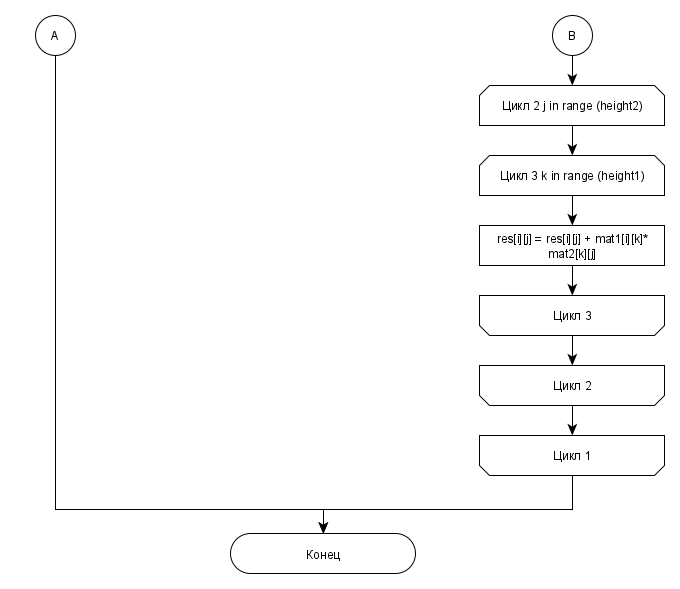
\includegraphics[width=0.8\linewidth]{basedab121.png}
		\caption{Стандартный алгоритм умножения матриц. Часть 2}
		\label{ris:std2}
	\end{figure}
	
	\newpage

	\begin{figure}[h!]
		\centering
		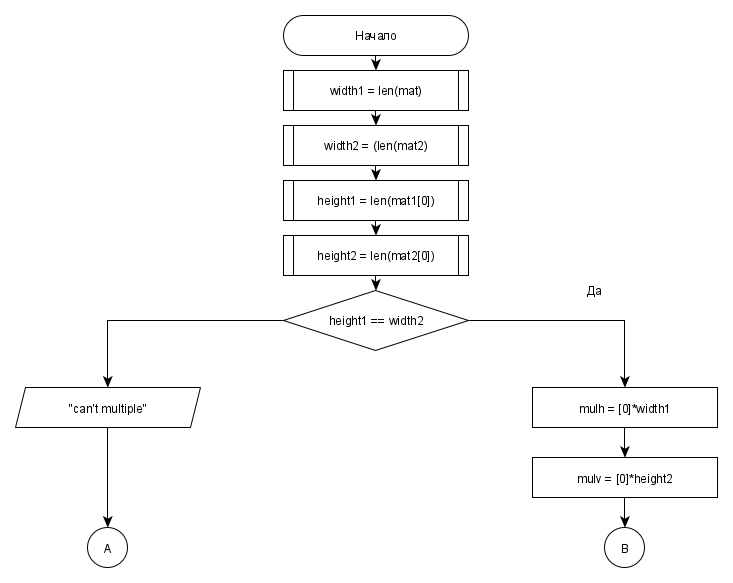
\includegraphics[width=1\linewidth]{part11.png}
		\caption{Алгоритм Винограда умножения матриц. Часть 1}
		\label{ris:wino1}
	\end{figure}
	
	\newpage
	
	\begin{figure}[h!]
		\centering
		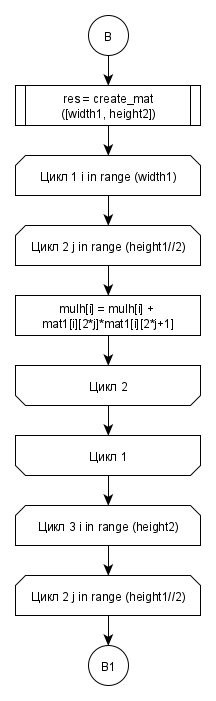
\includegraphics[width=0.4\linewidth]{part21.png}
		\caption{Алгоритм Винограда умножения матриц. Часть 2}
		\label{ris:wino2}
	\end{figure}

	\newpage

	\begin{figure}[h!]
		\centering
		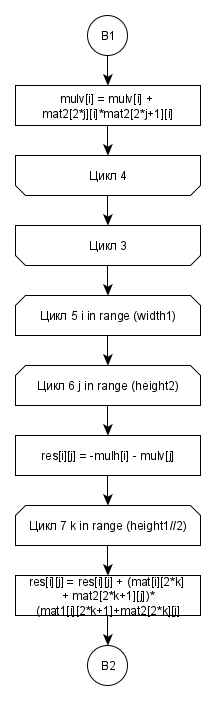
\includegraphics[width=0.4\linewidth]{part31.png}
		\caption{Алгоритм Винограда умножения матриц. Часть 3}
		\label{ris:wino3}
	\end{figure}

	\newpage
	
	\begin{figure}[h!]
		\centering
		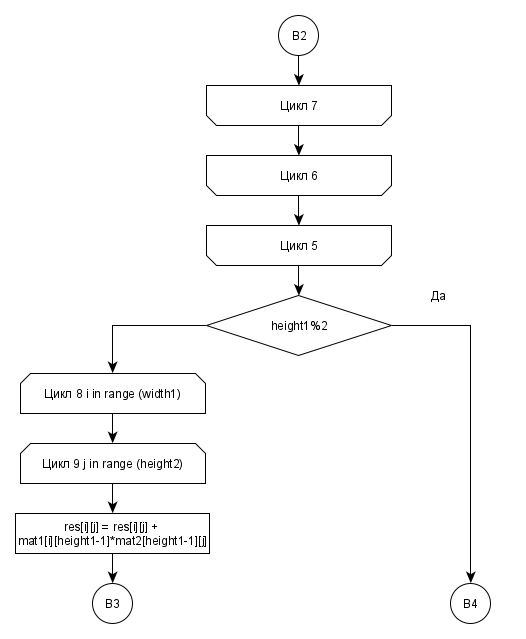
\includegraphics[width=0.8\linewidth]{part41.png}
		\caption{Алгоритм Винограда умножения матриц. Часть 4}
		\label{ris:wino4}
	\end{figure}

	\newpage

	\begin{figure}[h!]
		\centering
		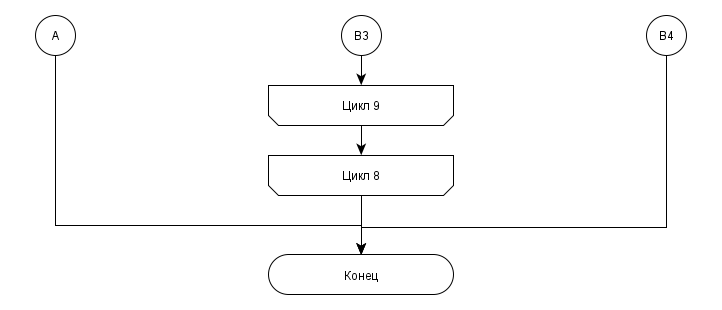
\includegraphics[width=0.8\linewidth]{part51.png}
		\caption{Алгоритм Винограда умножения матриц. Часть 5}
		\label{ris:wino5}
	\end{figure}
	
	\section{Вывод}

		В рамках раздела были рассмотрены схемы алгоритм умножения классически и по Винограду с целью их дальнейшего переноса в программу.

    \newpage

    \chapter{Технологическая часть}
        \label{sec:tecnologic_part}

        	В рамках раздела будут описаны инструментарии разработки, выбор среды, требования к ПО. 
        	Также будут предоставлены листинги конкретных реализаций алгоритмов.
        	
        	Замеры времени были произведены на: Intel(R) Core(TM) i3-6006U, 2 ядра, 4 логических процессоров.

	\section{Средства реализации}

        	Для реализации алгоритмов использовался язык программирования Python 3.8.0 и среда разработки PyCharm Community Edition 2019.3.1 by JetBrains. 
        	У меня есть определенный опыт работы с данным языком, которого будет достаточно для реализации текущей лабораторной работы, а среда разработки имеет бесплатную комьюнити версию и удобный интерфейс, упрощающий разработку приложения/скрипта.
        	
        	Замер времени реализован с помощью функции process\_time() библиотеки time.
        	Измеряется время исполнения кода чистого алгоритма (без учета времени на создание матриц, генерацию данных и т.п.).\\
		
	\section{Требования к программному обеспечению}

На вход программа должна получать две матрицы, для которых вычисляется их произведение тремя алгоритмами (стандартный алгоритм умножения матриц, алгоритм умножения матриц по Винограду, а также оптимизированный алгоритм умножения матриц по Винограду).

На выход программа должна выдавать результирующую матрицу всеми тремя алгоритмами, должна корректно обрабатывать исключительные ситуации вроде невозможности произведения данных матриц.

	\section{Листинг кода}

        	На листинге \ref{list:etc} представлены дополнительные функции и объявления, необходимые для реализации алгоритмов.
        	
        	На листинге \ref{list:wino} представлена реализация алгоритма Винограда.
        	
			На листинге \ref{list:wino_opt} представлена реализация оптимизированного алгоритма Винограда.

			На листинге \ref{list:std} представлена реализация стандартного алгоритма.
        
        \begin{lstlisting}[frame = single, breaklines, caption = Вспомогательные функции и объявления, label=list:etc]
	        import random
	        import time
	        
	        def print_matrix(mat):
	        	if mat:
	        		print("")
	        	for i in range (len(mat)):
	        		print(mat[i])
	        
	        def create_mat(size):
	        	width = size[0]
	        	height = size[1]
	        
	        	res = []
	        	for i in range (width):
	        		res.append([0]*(height))
	        
	        	return res
	        
	        def generate_mat(size):
	        	mat = create_mat(size)
	        	random.seed()
	        
	        	for i in range (size[0]):
	        		for j in range (size[1]):
	        			mat[i][j] = random.randint(0, 10)
	        
	        	return mat
	    \end{lstlisting}  
	   
	    \begin{lstlisting}[frame = single, breaklines, caption = Алгоритм Винограда, label=list:wino] 
	        def vinograd(mat1, mat2):
	        	width1 = len(mat1)
	        	width2 = len(mat2)
	        
	        	height1 = len(mat1[0])
	        	height2 = len(mat2[0])
	        
	        	if height1 != width2:
	        		print("\nCan't multiplex given matrixes")
	        		return
	        
	        	mulh = [0] * (width1)
	        	mulv = [0] * (height2)
	        
	        	res = create_mat([width1, height2])
	        	for i in range (width1):
	        		for j in range (height1//2):
	        			mulh[i] = mulh[i] + mat1[i][2*j] * mat1[i][2*j+1]
	        
	        	for i in range (height2):
	        		for j in range (height1//2):
	        			mulv[i] = mulv[i] + mat2[2*j][i] * mat2[2*j+1][i]
	        
	        	for i in range (width1):
	        		for j in range (height2):
	        			res[i][j] = -mulh[i] -mulv[j]
	        			for k in range (height1//2):
	        				res[i][j] = res[i][j] + (mat1[i][2*k]+
	        					mat2[2*k+1][j])*(mat1[i][2*k+1]+
	        					mat2[2*k][j])
	        
	        	if height1%2:
	        		for i in range (width1):
	        			for j in range (height2):
	        				res[i][j] = res[i][j] + mat1[i][height1-1] *
	        					mat2[height1-1][j]
	        
	        	return res
	    \end{lstlisting}
	        
	    \begin{lstlisting}[frame = single, breaklines, caption = Оптимизированный алгоритм Винограда, label=list:wino_opt]
	        def vinograd_optimized(mat1, mat2):
	        	width1 = len(mat1)
	        	width2 = len(mat2)
	        
	        	height1 = len(mat1[0])
	        	height2 = len(mat2[0])
	        
	        	if height1 != width2:
	        		print("\nCan't multiplex given matrixes")
	        		return
	        
	        	mulh = [0] * (width1)
	        	mulv = [0] * (height2)
	        	high_value = (height1//2)*2
	        
	        	res = create_mat([width1, height2])
	        	for i in range (width1):
	        		for j in range (0, high_value, 2):
	        			mulh[i] -= mat1[i][j]*mat1[i][j+1]
	        
	        	for i in range (height2):
	        		for j in range (0, high_value, 2):
	        			mulv[i] -= mat2[j][i]*mat2[j+1][i]
	        
	        	for i in range (width1):
	        		for j in range (height2):
	        			res[i][j] = mulh[i] + mulv[j]
	        
	        			buffer = 0
	        			for k in range (0, high_value, 2):
	        				buffer += (mat1[i][k]+mat2[k+1][j])*
	        					(mat1[i][k+1]+mat2[k][j])
	        			res[i][j] += buffer
	        
	        			if height1 % 2:
	        				res[i][j] += mat1[i][height1-1]*
	        					mat2[height1-1][j]
	        
	        	return res
	    \end{lstlisting}
	    
	    \begin{lstlisting}[frame = single, breaklines, caption = Стандартный алгоритм умножения матриц, label=list:std]
	        def based(mat1, mat2):
	        	width1 = len(mat1)
	        	width2 = len(mat2)
	        
	        	height1 = len(mat1[0])
	        	height2 = len(mat2[0])
	        
	        	if height1 != width2:
	        		print("\nCan't multiplex given matrixes")
	        		return
	        
	        	res = create_mat([width1, height2])
	        	for i in range (width1):
	        		for j in range (height2):
	        			for k in range (height1):
	        				res[i][j] = res[i][j] + mat1[i][k]*mat2[k][j]
	        
	        	return res
        \end{lstlisting}
        
    \section{Вывод}

        	В рамках раздела были предъявлены требования к программному обеспечению. 
        	На основании их были разработаны и представлены конкретные реализации всех трёх алгоритмов умножения матриц.

    \newpage

    \chapter{Экспериментальная часть}
        \label{sec:experimental_part}

        	В рамках раздела на рисунках \ref{ris:work1}-\ref{ris:work2} будут представлены результаты работы программы. 
        	Будут проведены эксперименты по вычислению времени выполнения алгоритмов, результаты которых представлены на рисунке \ref{ris:test1}.

	\section{Примеры работы}

        \begin{figure}[h!]
        	\centering
        	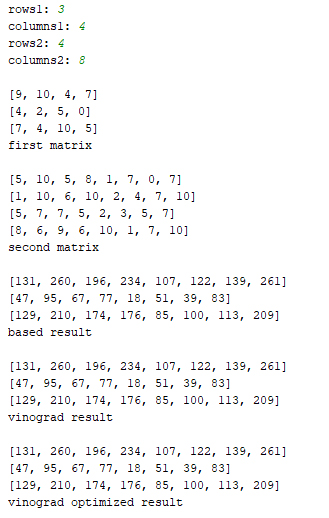
\includegraphics[width=0.5\linewidth]{test_mult1.jpg}
        	\caption{Результат работы программы при корректных исходных данных}
        	\label{ris:work1}
        \end{figure}
        
        \newpage
        
        \begin{figure}[h!]
        	\centering
        	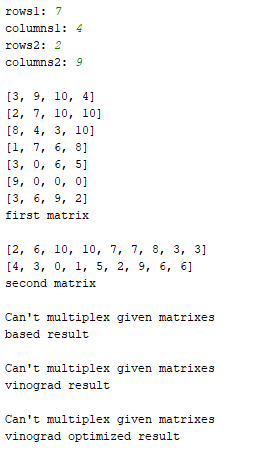
\includegraphics[width=0.7\linewidth]{test_mult2.jpg}
        	\caption{Результат работы программы при некорректных исходных данных}
        	\label{ris:work2}
    	\end{figure}
        
        \newpage
        
    \section{Сравнительный анализ на основе экспериментальных данных}

        	В ходе эксперимента был проведен замер времени для всех реализаций алгоритмов на размерностях матриц 100х100,...,1000х1000 и 101х101,...,1001х1001.
        
        \begin{figure}[h!]
        	\centering
        	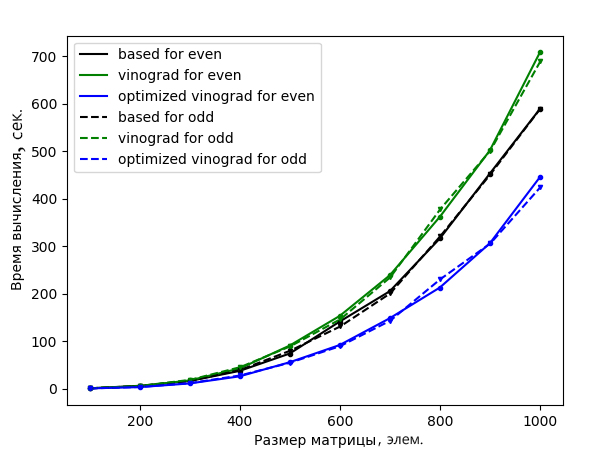
\includegraphics[width=0.8\linewidth]{graph_mult.jpg}
        	\caption{Сравнение времени выполнения алгоритмов на разных входных данных}
        	\label{ris:test1}
        \end{figure}
        
    \section{Оценка трудоёмкости}

        	Считаем, что перемножаются матрицы размерами (width1, height1) и (width2,height2), height1 == width2 в случае выполнения произведения.

    \subsection{Модель оценки трудоёмкости}

        	Введём систему оценки трудоемкости.
        	\begin{enumerate} 
	        	\item Объявление переменной/массива без определения имеет трудоёмкость 0\\
	        	\item Операторы +,-,*,/,=, а также +=,-=,// имеют трудоёмкость 1\\
	        	\item Оператор доступа по индексу [] имеет трудоёмкость 1\\
	        	\item Логические операции имеют трудоёмкость 1\\
	        	\item Цикл имеет трудоёмкость 2+n(2+t), где n - кол-во итераций, t-трудоёмкость тела цикла	
        	\end{enumerate}
	
	\newpage

	\subsection{Стандартный алгоритм}

        	Расчёт трудоёмкости для стандартного алгоритма.
        	\begin{multline*}
        		F = 2+width1*(2+2+height2*(2+2+height1*(2+8+1+1+1))) = \\ 2+width1*(4+height2*(4+13*height1)) = \\2+width1*(4+4*height2+13*height2*height1) =\\ 2+4*width1+4*width1*height2+13*width1*height1*height2 \sim O(n^{3})
        	\end{multline*}

	\subsection{Алгоритм Винограда}

        	Расчёт трудоёмкости для алгоритма Винограда.
        	\begin{multline*}
        		F_{1} = 2+width1*(2+3+height1//2*(3+6+1+2+3)) = \\2 + width1*(5+height1//2*(15)) =\\ 2+width1*(5+15*height1//2) =\\ 2+5*width1+15*width1*height1//2
        	\end{multline*}
        	
        	\begin{multline*}
        		F_{2} = 2+height2*(2+3+height1//2*(3+6+1+2+3)) = \\2 + height2*(5+height1//2*(15)) =\\ 2+height2*(5+15*height1//2) =\\ 2+5*height2+15*height2*height1//2
        	\end{multline*}
        	
        	\begin{multline*}
        		F_{3} = 2+width1*(2+2+height2*(2+4+1+2+3+height1//2*(3+12+1+5+5))) = \\2 + width1*(4+height2*(12+26*height1//2)) =\\ 2+width1*(4+12*height2+26*height2*height1//2) =\\ 2+4*width1+12*width1*height2+26*width1*height2*height1//2
        	\end{multline*}
			
			\begin{multline*}
				F_{4} = 
				\left[ 
					\begin{gathered} 
						1\\
						3+width1*(2+2+height2*(2+8+1+3+1))\\ 
			 		\end{gathered} 
		 		\right] =\\
		 		\left[ 
		 			\begin{gathered} 
		 				1\\
		 				3+width1*(4+height2*(15))\\ 
		 			\end{gathered} 
		 		\right] =\\
		 		\left[ 
		 			\begin{gathered} 
		 				1\\
		 				3+4*width1+15*width1*height2\\ 
		 			\end{gathered} 
		 		\right]
	 		\end{multline*}
	 		
	 		\begin{multline*}
	 			F = 2+5*width1+15*width1*height1//2+\\
	 			2+5*height2+15*height2*height1//2+\\
	 			2+4*width1+12*width1*height2+26*width1*height2*height1//2+\\
	 			\left[ 
	 				\begin{gathered} 
	 					1\\
	 					3+4*width1+15*width1*height2\\ 
	 				\end{gathered} 
	 			\right] \sim O(n^{3})
	 		\end{multline*}
	 		
	\newpage
	 		
    \subsection{Оптимизированный алгоритм Винограда}

        	Расчёт трудоёмкости для оптимизированного алгоритма Винограда.
        	\begin{multline*}
        		F_{1} = 2+width1*(2+2+height1//2*(2+5+1+1+1)) = \\2+width1*(4+height1//2*(10)) =\\ 2+width1*(4+10*height1//2) =\\ 2+4*width1+10*width1*height1//2
        	\end{multline*}
        	
        	\begin{multline*}
        		F_{2} = 2+height2*(2+2+height1//2*(2+5+1+1+1)) = \\2+height2*(4+height1//2*(10)) =\\ 2+height2*(4+10*height1//2) =\\ 2+4*height2+10*height2*height1//2
        	\end{multline*}
        	
        	\begin{multline*}
        		F_{3} = 2+width1*(2+2+height2*(2+4+1+1+1+
        		\left[ 
        			\begin{gathered} 
        				1\\
        				6+1+2+1\\ 
        			\end{gathered} 
        		\right] +height1//2*(2+8+1+4+1))) = \\2+width1*(4+height2*(14+
        		\left[ 
        			\begin{gathered} 
        				1\\
        				10\\ 
        			\end{gathered} 
        		\right] +16*height1//2)) =\\ 2+width1*(4+height2+
        		\left[ 
        			\begin{gathered} 
        				height2\\
        				10*height2\\ 
        			\end{gathered} 
        		\right] + 16*height2*height1//2 =\\ 2+4*width1+14*width1*height2+
        		\left[ 
        			\begin{gathered} 
        				width1*height2\\
        				10*width1*height2\\ 
        			\end{gathered} 
        		\right] +16*width1*height2*height1//2
        	\end{multline*}
        	
        	\begin{multline*}
        		F = 2+4*width1+10*width1*height1//2+\\
        		2+4*height2+10*height2*height1//2+\\
        		2+4*width1+14*width1*height2+
        		\left[ 
        			\begin{gathered} 
        				width1*height2\\
        				10*width1*height2\\ 
        			\end{gathered} 
        		\right] +16*width1*height2*height1//2 \sim O(n^{3})
        	\end{multline*}

	\section{Выполненная оптимизация}

        	\begin{enumerate}
	    		\item height1//2 заменено на height1//2*2, в связанных циклах последовали соответствующие изменения:\\
	    		\begin{itemize}
	    			\item в циклах заполнения вспомогательных массивов mulh и mulv 2*j заменено на j\\
	    			\item в основном цикле умножения матриц 2*k заменено на k\\
	    		\end{itemize}
	    		\item Работа со значениями матрицы производится через буферную переменную\\
	    		\item Условие на проверку нечетной размерности результирующей матрицы перенесено из отдельного вложенного цикла в основной вложенный цикл 
	    	\end{enumerate}
    	
    \section{Вывод}

        Алгоритм умножения матриц по Винограду работает быстрее, чем его аналог в лице стандартного алгоритма. 
        Выигрыш во времени достигается путем введения двух дополнительных массивов и тем самым снижением числа умножений, причем разница составляет до 45\% в пользу оптимизированного алгоритма Винограда. 
        На нечетных размерностях матриц может происходить нивелирование преимущества за счет дополнительных проверок и траты ресурсов на обработку последней строки/столбца, причем разница составляет не более 5\%. 

    \newpage

    \chapter*{Заключение}
        \label{sec:conclusion_part}

			В результате выполнения данной работы был реализован классический алгоритм умножения матриц. 
			Был изучен и реализован алгоритм Винограда. 
			Был разработан и реализован оптимизированный вариант алгоритма Винограда. 
			Была выбрана модель оценки трудоёмкости и по ней были даны оценки трудоёмкости классическому алгоритму умножения матриц, алгоритму Винограда (для лучшего и худшего случая) и оптимизированному алгоритму Винограда (для лучшего и худшего случая). 
			Проведены замеры времени для алгоритмов. 
			
			В ходе экспериментов выяяснилось, что алгоритм Винограда работает до 45\% быстрее по сравнению со стандартным алгоритмом. 
			
			Разница между лучшим и худшим случаями алгоритма Винограда составляет до 5\% на тестовых размерностях до 1001x1001.
       
    \begin{thebibliography}{2}
    	\bibitem{Beloysov}
    	И. В. Белоусов(2006), Матрицы и определители, учебное пособие по линейной алгебре, с. 1 - 16
    	\bibitem{Gall2012}
    	Le Gall, F. (2012), "Faster algorithms for rectangular matrix multiplication", Proceedings of the 53rd Annual IEEE Symposium on Foundations of Computer Science (FOCS 2012), pp. 514–523
    	%https://arxiv.org/pdf/1204.1111.pdf
    \end{thebibliography}
       
\end{document}
